\documentclass{beamer}

\usepackage{amsmath}
\usepackage[style=alphabetic,url=true]{biblatex}
\usepackage{environ}
\usepackage{geometry}
\usepackage{graphicx}
\usepackage{tikz}
\usepackage[T2A]{fontenc}
\usepackage[utf8]{inputenc}
\usepackage{listings}

\graphicspath{ {./graphics/} }
\usetikzlibrary{shapes.arrows,chains}
\usecolortheme{beaver}
\setbeamertemplate{itemize item}[circle]
\setbeamertemplate{itemize subitem}{--}
\addtobeamertemplate{navigation symbols}{}{
  \usebeamerfont{footline}
  \usebeamercolor[fg]{footline}
  \hspace{1em}
  \insertframenumber/\inserttotalframenumber
}


\title{
  Common Lisp and Introduction to Functional Programming \\
  Lecture 1: Introduction
}
\author{Yuri Zhykin}
\date{Feb 4, 2021}

\begin{document}

\frame{\titlepage}

\begin{frame}
  \frametitle{Contacts}
  \begin{itemize}
    \item @rodentrabies on Telegram
    \item https://github.com/rodentrabies
  \end{itemize}
\end{frame}

\begin{frame}
  \frametitle{Course structure 1/2}
  \begin{itemize}
  \item Basic concepts
    \begin{itemize}
    \item Intensional vs. extensional ways of viewing things
    \item Turing's vs. Church's views of computations
    \item Imperative vs. declarative approaches to programming
    \end{itemize}
  \item Introduction to Common Lisp
    \begin{itemize}
    \item Short introduction to $\lambda$-calculus 
    \item Language primitives
    \item Detailed study of Lisp functions
    \item Common Lisp Object System (CLOS)
    \item Discussion of Lisp's homoiconicity and macros
    \end{itemize}
  \item Functional programming basics
    \begin{itemize}
    \item Functions, state, mutation, procedures
    \item Referential transparency
    \item Recursion and composition of functions
    \item Functions as first class objects in programming languages
    \item When and why functional approach is better
    \end{itemize}
  \item[] ...
  \end{itemize}
\end{frame}

\begin{frame}
  \frametitle{Course structure 2/2}
  \begin{itemize}
  \item[] ...
  \item Case study: sequence processing with recursive operators
    \begin{itemize}
    \item Map, Reduce and Filter
    \end{itemize}
  \item ``Advanced'' functional programming
    \begin{itemize}
    \item Introduction to type theory
    \item Type inference
    \item Purely functional programming languages
    \item Lazy evaluation
    \item Introduction to category theory
    \item Interactive theorem provers
    \end{itemize}
  \item Other declarative programming paradigms
    \begin{itemize}
    \item Constraint programming
    \item Domain-specific languages
    \item Logic programming
    \end{itemize}
  \end{itemize}
\end{frame}

\begin{frame}
  \frametitle{Intensional and extensional definitions}
  \begin{itemize}
  \item \textbf{Intensional} definition states \textit{necessary and sufficient
      conditions} for the concept to be applied
    \begin{itemize}
    \item ``Actor is a person that portrays a character in a performance.''
    \end{itemize}
  \item \textbf{Extensional} definition provides \textit{a set of all instances}
    of the concept being applied
    \begin{itemize}
    \item ``Actors: Ryan Gosling, Harrison Ford, Rutger Hauer...''
    \end{itemize}
  \item Intensional definitions deal with internals of the concept
  \item Extensional definitions ignore internals of the concepts
  \end{itemize}
\end{frame}

\begin{frame}
  \frametitle{Turing, Church and computable functions}
  \begin{itemize}
  \item Kurt G\"{o}del, 1933: general recursive functions
  \item Alan Turing, 1936: Turing-computable functions - all functions that can
    be computed by a Turing machine
  \item Alonzo Church, 1936: $\lambda$-computable function - all functions that
    can be described by a term of the $\lambda$-calculus
  \item Church-Turing, 1936-1937: function is $\lambda$-computable iff it is
    Turing-computable and iff it is general recursive
  \end{itemize}
\end{frame}

\begin{frame}[fragile]
  \frametitle{Imperative programming}
  \begin{itemize}
  \item Imperative programming describes \textbf{how} to achieve the final result
    by sequentially executing a set of primitive steps
  \item Steps explicitly modify the state of the program
  \item Turing machine is the simplest imperative programming model
    \begin{itemize}
    \item clearly defined state
    \item a set of instructions to be executed
    \end{itemize}
  \end{itemize}
  \begin{center}
    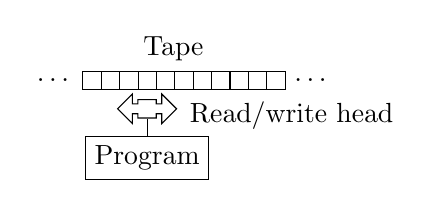
\begin{tikzpicture}[start chain=1 going right,start chain=2 going below,node distance=-0.15mm]
      \node [on chain=2] {Tape};
      \node [on chain=1] at (-1.5,-.4) {\ldots};  
      \foreach \x in {1,2,...,11} {
        \x, \node [draw,on chain=1] {};
      } 
      \node [name=r,on chain=1] {\ldots}; 
      \node [name=k, arrow box, draw,on chain=2, arrow box arrows={east:.25cm, west:0.25cm}] at (-0.335,-.65) {};    
      \node at (1.5,-.85) {Read/write head};
      \node [on chain=2] {};
      \node [draw,on chain=2] {Program};
      \chainin (k) [join];
    \end{tikzpicture}
  \end{center}
\end{frame}

\begin{frame}
  \frametitle{Declarative programming}
  \begin{itemize}
  \item Declarative programming defines \textbf{what} the final result is and
    leaves the ``how'' to the implementation of the programming environment
  \item Since there are no steps that modify the state, there is no explicit
    state                       
  \item Declarative programming is often described as any programming that is
    not imperative:
    \begin{itemize}
    \item markup languages (HTML)
    \item query languages (SQL, SPARQL)
    \item logic programming (Prolog)
    \item functional programming (building programs out of composable functions)
    \end{itemize}
  \end{itemize}
\end{frame}

\begin{frame}
  \frametitle{Why is declarative programming important?}
  \begin{itemize}
  \item Programs written declaratively are easier to read and analyze, since
    there is no need to keep the state in mind
  \item Computers are much better at keeping lots of details in memory than
    humans, and declarative programming leaves maintaining of state to the
    programming environment
  \item Most of modern programming languages provide tools for functional
    programming, and these tools are often the best tools for the job, so
    learning to use these tools properly is essential to writing idiomatic
    programs in modern languages
  \end{itemize}
\end{frame}

\begin{frame}
  \frametitle{The end}
  \begin{center}
    Thank you!
  \end{center}
\end{frame}

\end{document}
